\chapter{From corrective to predictive process control} \label{From Corrective to Predictive Process Control}
\minitoc

\section{Introduction}

In this chapter, we propose a data-driven approach for improving process control. The objective is to build a statistical model of the relationship between the process conditions and the  quality of the parts produced under these conditions. Firstly, it is necessary to have a representative data set of the phenomenon to be modeled. Then, the statistical model must be selected. An application of this approach to the extrusion blow-molding process will be presented in section \ref{Empirical Setting}. Finally, it is under the prism of industrial constraints that we will discuss the limits to the deployment of these methods on production lines.


\section{Motivation}

Poor quality or ``scrap'' parts are very expensive for a company like Plastic Omnium Clean Energy Systems. The “Cost of Non-Quality” (CNQ) is one of the key indicators most used by the company. However, when a part is bad, it is first necessary to understand the origin of the problem, which can require a lot of time and energy. Historically, our industrial process monitoring has been driven using a knowledge-based corrective approach (Figure \ref{fig:Corrective process control}). The quality measurements of each product is used to adjust the process and to maintain the process capability. Moreover, some of the process parameters, which are considered as critic for process safety, are kept under control through the use of uni-variate control charts.  When a parameter falls outside the control limits, some warning messages are generated to alert the operators who have the task of regulating the machine so that the parameter can return in the safe zone. 

\begin{figure}
\centerline{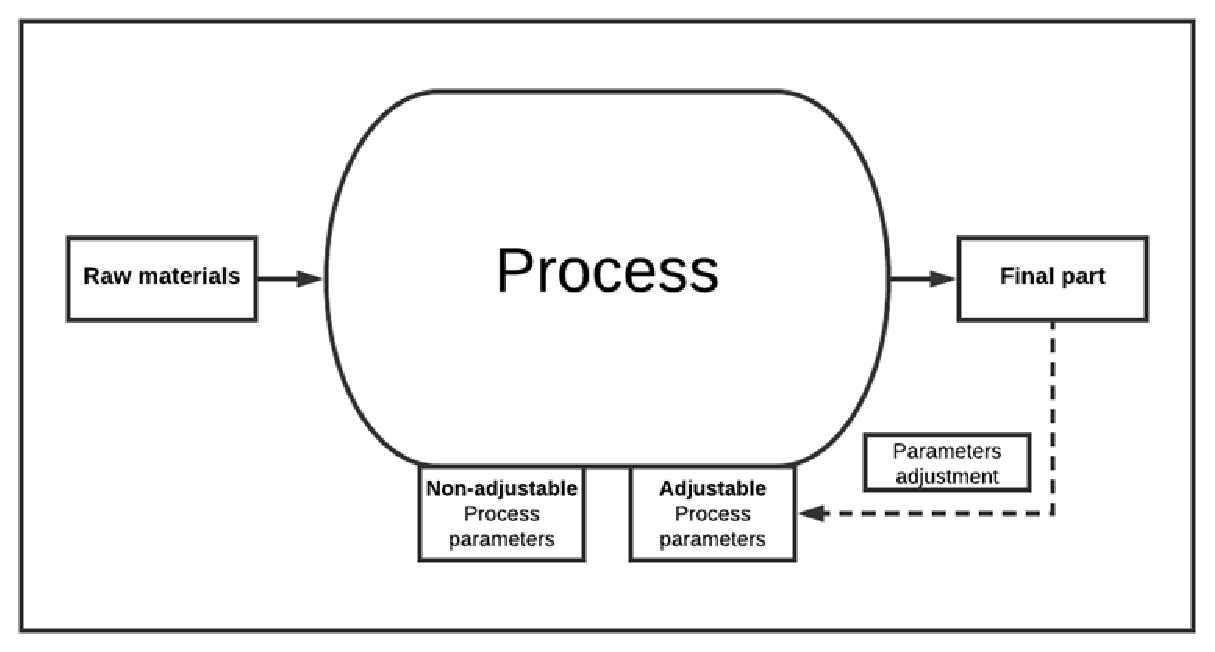
\includegraphics[scale=0.7]{images/chapter_3/corrective_approach.eps}}
\caption{Corrective process control}
\label{fig:Corrective process control}
\end{figure}

Evidence has shown how the overall process stability ensures, in most cases, the product quality stability. However, it still remains unclear how the system parameters affect the product quality variability. Moreover, quality prediction can offer the possibility to define better system parameters at an early production stage. In other words, the product quality anticipation may be used to adjust the process in real time and not retrospectively (Figure \ref{fig:Predictive process control}). Such an approach would allow the product failure anticipation and the just-in-time process correction with an overall reduction of the non-conforming parts.

\begin{figure}
\centerline{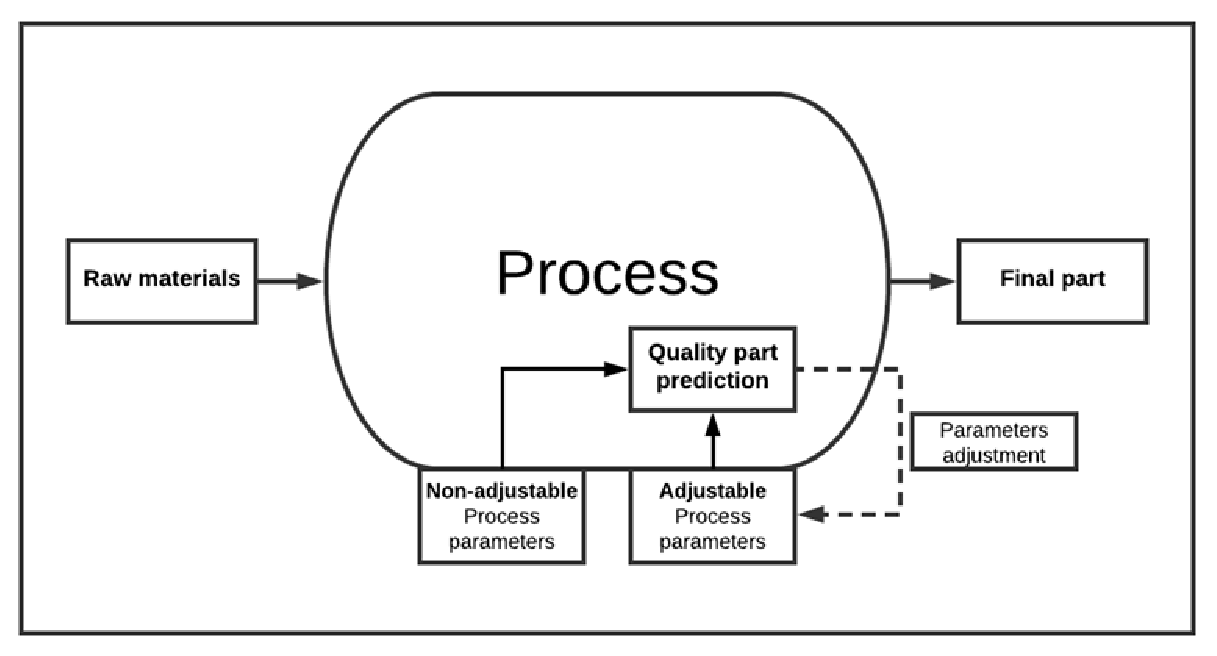
\includegraphics[scale=0.7]{images/chapter_3/predictive_approach.eps}}
\caption{Predictive process control}
\label{fig:Predictive process control}
\end{figure}

In order to understand the relationship between process parameters and the quality of final part, we use a supervised learning approach. We view our complex industrial process as a black box with multiple inputs and one output. Given $p$ process parameters $(X_1,X_2,\ldots,X_p)$ and one product quality variable $Q$, we look for the function that better approximates the relationship between the inputs and the output. Mathematically speaking, we look for the function $\hat{f}$ that approximates the relationship between the process variables and the quality result so that the following expression is verified:

\begin{equation}
    Q = \hat{f}(X_1,X_2,\ldots,X_p) + \epsilon
    \enspace,
\end{equation}
where $\epsilon$ is

By an automatic analysis of a set of examples (training set) of measured input-output behaviour of the process learning algorithms can find out important causal relationships between process variables and construct classifiers for detecting dangerous or unwanted process states.


\section{Proposed method} \label{Proposed Method}

In this section, we will try to define a general framework that can be applied to improve process control. We use supervised machine learning to discover some patterns between the process parameters and the quality of the part that has been manufactured by the same process. We proceed in four main stages:
\begin{enumerate}
    \item \textit{Data collection} consist in retrieving all the data needed to model the manufacturing production process. It involves two main stages:  data acquisition and  data labelling (Section \ref{Data Collection}). 
    \item \textit{Data processing} covers the range of operations required to make the input data suitable for the machine learning algorithm (Section \ref{Data Processing}). 
    \item \textit{Exploratory data analysis} is an ensemble of simple graphical and quantitative techniques that can be used to explore data and retrieve important information (Section \ref{Exploratory Data Analysis}).
    \item \textit{Data modelling} corresponds to the statistical modelling of the relationship between the input process data and the output quality data by a machine learning algorithm (Section \ref{Machine Learning modeling})
\end{enumerate}
%
\begin{figure}
\centerline{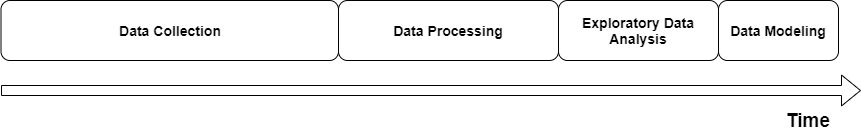
\includegraphics[scale=0.45]{images/chapter_3/stages.png}}
\caption{The 4 stages towards predictive process control}
\label{fig:4_stages}
\end{figure}
%
In the remaining part of the current section we will review in details how to carry out these four steps to achieve a \textit{predictive process control}. 

\subsection{Data collection} \label{Data Collection}

Collecting data allows to capture a record of past events so that we can use data analysis to find recurring patterns. In the context of this research work, the data collection is the task of retrieving the data that could be meaningful to explain the variability of a quality characteristic given some process parameters. Among the many challenges in Industry 4.0, data collection is becoming one of the critical bottlenecks. It is known that the majority of the time for building end-to-end data-driven models is spent on preparing the data, which includes collecting, cleaning, analyzing, visualizing, and feature engineering. Moreover, as machine learning is used in new applications, it is usually the case that there is not enough training data. Traditional applications of machine learning like machine translation or image object detection rely on huge quantities of training data that have been accumulated for decades. On the other hand, more recent applications, especially in the manufacturing industry, have little or no training data. To train a machine learning model, it is necessary to have samples that are representative of the entire operating range of the process. If the individuals do not cover the whole process functioning, the model will be biased.

Two kind of data are required: the input data, corresponding to the process data and the output data which is actually the measure of the quality of the parts. Data collection involves mainly two different steps: \textit{process data acquisition} and \textit{Quality data acquisition}. 

\subsubsection{Process data acquisition} \label{Process Data Acquisition}

In this PhD dissertation we define \textit{process data} any kind of data belonging to the manufacturing process taken into account. For instance, some of the process parameters of the extrusion blow-molding process are the extruder throughputs, the extruder temperature, as well as the air blowing pressure. These process data constitute a picture of the state of the process at a given time.

Process data acquisition is a challenging task in Industry 4.0 due to different technologies, machines, sensors, IoT devices and communication networks. Sensors, actuators, and PLCs are the main data generator in the automotive industry \citep{khan2017big}. In the last decade a new type of intelligent sensors, also called \textit{Smart Sensors}, are more and more used in the manufacturing industry. Most of the data available in the Manufacturing plants comes from PLCs, Sensors and Smart Sensors. The three devices are further explained as below.

\begin{itemize}
    \item \textit{Sensors}: A sensor is a device that converts a physical state or activity into an electrical signal. This electrical signal is sent to the PLC for further processing. In manufacturing, sensors create a huge amount of data. Most machines and robots include sensors that collect data from their surroundings, such as temperature sensors, which are used to detect the heat of a machine or the environment.
    \item \textit{Smart sensors}: With the developments of the IOT and machine learning, are today available in the market various types of Smart Sensors. Smart sensors are devices that take information from a physical environment and use embedded microprocessors and wireless communication to monitor, examine and provides information about the proper functioning of the observed system. These sensors are today massively applied in the manufacturing industry and they provides a lot of information that can be used in the task of better controlling the process and to better understand the quality part variability.
    \item \textit{Actuators}: The actuator takes an electrical signal from the PLC and turns it into physical action. A basic example of an actuator connected to a PLC is the automatic starting of a motor. There are several robots for automated procedures in the industrial business. These robots are actuators that produce a large quantity of data.
    \item \textit{PLC}: PLC is a programmable unit where the instructions for automation are stored and takes a decision based on the input data from the sensors while actuators work on the PLC instructions (Figure \ref{fig:plc}). A factory has a lot of PLCs based on the processes. PLCs are made by different vendors and it generates heterogeneous data which is a big challenge for industrial big data.
    A plant has a large number of PLCs. PLCs are manufactured by many vendors and create heterogeneous data, which is a big challenge for industrial big data.
\end{itemize}

\begin{figure}
\centerline{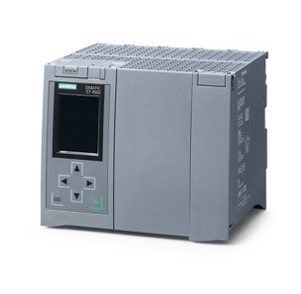
\includegraphics[scale=1]{images/chapter_3/PLC.jpg}}
\caption{PLC \textit{Siemens} S7-1500}
\label{fig:plc}
\end{figure}


The presented devices produces a lot of data but they do not manage the data storage. In fact, PLCs have a limited amount of storage space and they cannot be used to store the data permanently. The local machine data storage is most of the time handled by the SCADA (Supervisory Control And Data Acquisition) software. The term SCADA is used to identify any kind of software, installed on a personal computer or server, which allows the implementation, operation and management of supervisory, control and remote control systems without necessarily having to write code using programming languages. SCADA software have multiples functionalities which range from automation, to alarm handling, logging, archiving and simple statistical analysis \citep{daneels1999scada}. SCADA is a powerful system for acquisition of industrial automation data but, it is not able to handle the storage of a large volume of data. For this reason the collected data through the SCADA system should be stored elsewhere, in a place where data are easily accessible. Cloud platform, whether they are internal the manufacturing company or outside, are generally the solution for storing a large amount of data. Cloud platforms, or \textit{data Lake}, has been designed to be highly scalable and it provides a way to easily access the data through Big data technology that facilitate and accelerate the data analysis stages.  

In order to be able to properly manage the data acquisition, taking into account the heterogeneity of the data coming from the different data sources, we propose to introduce a \textit{Gateway} system which constitutes an intermediary bridge between the shop floor PLCs, ans sensors, and the Cloud platform where the data are stored. Moreover, it can communicate with the \textit{MES} system. The Manufacturing Execution System (MES) is a production management system serving as the information center in the enterprise to improve manufacturing transparency. It is the middle layer connecting the manufacturing process on the shop floor and the business process on the Enterprise Resource Planning (ERP) \citep{chen2020implementation}. By communicating with the MES system, it is possible to associate to a produced part the set of events that have enabled its production.

The architecture of the overall data acquisition system is visible in Figure \ref{fig:data_acquisition_architecture}.

\begin{landscape}
\begin{figure}
\centering
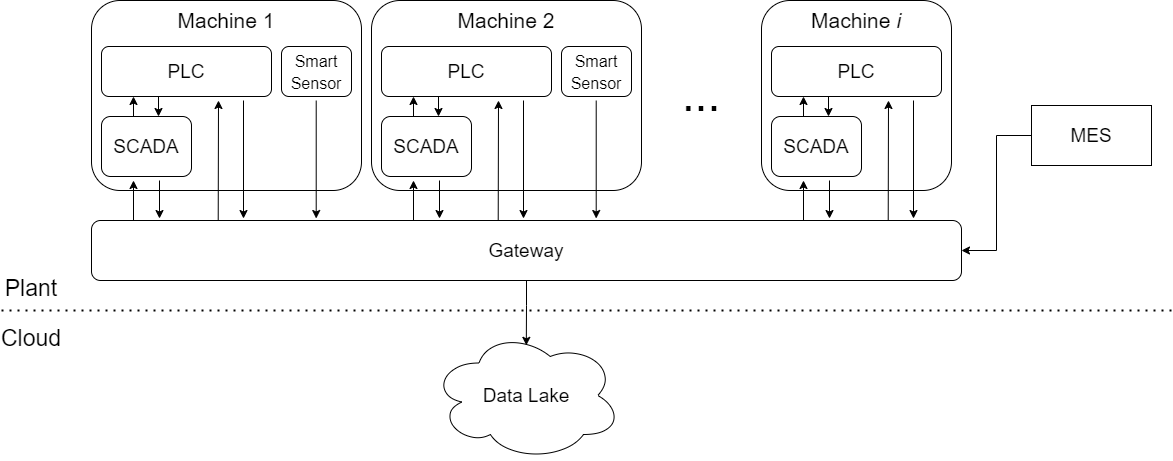
\includegraphics[scale=0.5]{images/chapter_3/Data_acquisition_architecture.png}
\caption{Data acquisition architecture}
\label{fig:data_acquisition_architecture}
\end{figure}
\end{landscape}

The gateway is a physical or virtualized server which acts like an intermediary between the data acquisition systems available in the shop floor and the Cloud platform where the data are stored for data analysis. The gateway connected to the shop floor network and it is able to interact directly with the PLC of the machines as well as smart sensors.  

The gateway has two main roles:

\begin{itemize}
    \item It allows to centralize the data collection at the plant level. It is in charge to retrieve the data from all the data sources, whether they are PLCs, Smart Sensors, SCADA software or the MES system. This process facilitates the subsequent sending of data to the Cloud platform. 
    \item This gateway is well suited for eventually deploying in production at the plant side the machine learning models that have been trained. 
\end{itemize}

The gateway should be equipped with different tools and software to allows the communication with the machines through the different communication protocols mainly used in Industry 4.0. There exist a multitude of communication protocols. Among all these we can mention \textit{OPC UA} and \textit{MQTT}. OPC UA (Open Platform Communications Unified Architecture) is a service-oriented machine-to-machine communication protocol mainly used in industrial automation. Its main goals are to provide a cross-platform communication protocol while using an information model to describe the transferred data \citep{profanter2019opc}. MQTT (Message Queuing Telemetry Transport) is an open message protocol which mainly focuses on a small code footprint and low network bandwidth usage, while handling high latency or bad network connections \citep{profanter2019opc}. Further information regarding the communication protocols used in Industry 4.0 are available in \citep{profanter2019opc}\citep{8262021}\citep{zezulka2018communication}.


\paragraph{Process data types}

When dealing with process data, we distinguish two different types of data: \textit{Cyclical data} and \textit{Time series data}.

\begin{itemize}
    \item \textit{Cyclical data}: Cyclical data are scalar values which provide information about a certain recurring event. Examples of Cyclical data are the machine cycle time, or the time needed from the machine to perform an operation. 
    \item \textit{Time series data}: Whenever a production process, or a part of it, requires time to be completed, it is possible to recover multiple sequential values of the same process parameters. This sequence of sequential data take the name of time series. The number of sequential values composing the time series depends on the sampling rate and may change accordingly to the nature of the measurement. For instance, the temperature of a machine components may be measured all along the production cycle and it is a classical example of time series data.
\end{itemize}

\begin{figure}
\centering
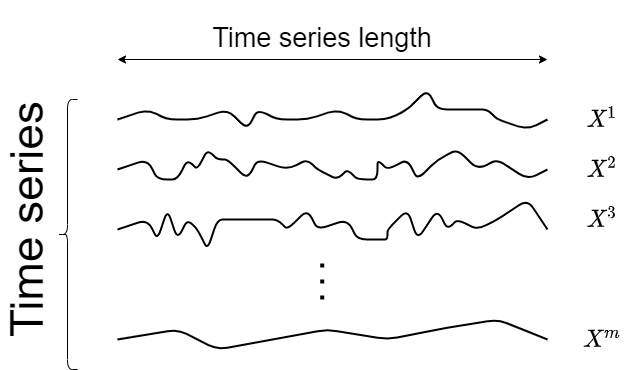
\includegraphics[scale=0.5]{images/chapter_3/time_series_data.png}
\caption{Time series data}
\label{fig:time_series_data}
\end{figure}


\subsection{Quality data acquisition}

Quality data acquisition is the task of collecting product quality data associated with all or some of the parts produced. The quality label can be continuous or discrete depending on the applied measurement method. For instance, we can measure a thickness of a manufactured part and provides the results in the form of continuous values in meters. On the other hand, we can measure a thickness value and associate it to  a class according to its compliance, or non-compliance with the specifications. Accordingly to the type of the label, either discrete or continuous, the data modelling may change. If the label is discrete the supervised learning modelling takes the form of a Classification problem (\ref{Classification}), otherwise it will be treated as a Regression problem (\ref{Regression}).   

The quality data acquisition can be done offline or online. The following two paragraphs will provide an overview of these two methods. 


\paragraph{Offline acquisition}

Offline acquisition, is the most common approach for labelling manufacturing data. In fact, for all non-visual product characteristics, it is extremely complicated to asses the quality of a part in less then a minute. Most of the quality controls realized on the part require specific equipment and the task of controlling the part can take several minute. Moreover, effective controlling might result in the destruction of the product or render it unfit for sale in some way. In such a case, the only possibility is to measure the quality of the part offline. Measuring offline has the advantage of allowing careful control of the manufactured parts, reducing the possibility of measurement error. However, as there are only a few parts to measure, it may takes a long time to build a dataset which is representative of all categories of part non-compliance.

Since, we are not able to measure the quality of all parts produced, it becomes crucial to structure the data collection to make them easily usable for future data analysis. Data have to be stored in a database and the quality measurement must be related to a part number, or traceability number, in order to subsequently associate it with the process data, which in turn must be tagged with the part number. 


\paragraph{Online acquisition}

Performing the online data acquisition, on the production line, eliminates two critical error risks:
\begin{enumerate}
    \item The loss of the link between the production measurements and the off-line annotation.
    \item The transformation of the parts between their production and their annotation.
\end{enumerate}

On the other hand, the time available for the annotation is very limited. Most of the time the machine operators have time constraints to meet the production cadence. As a consequence this data annotation must be done in a limited amount of time. Depending on the operator task the available time for performing the control may change. We estimate that the operator can consecrate a maximum of one third of the production cycle time to this task, which means that for a process with a cadence of 60 seconds the operator has at maximum 20 seconds to perform this task. In addition to the annotation time, the human expert has to assist in the handling of the parts and related operations.

By automating the process data acquisition through the data collection presented above, and by ensuring the proper registration of the quality data obtained by measuring the parts, it is possible to permanently feed a dataset with new data in an automatic manner. Over time we can hope to recover enough data to cover the all distribution of all possible quality non-conformities. 

\subsection{Data processing} \label{Data Processing}

As heterogeneous data is collected in manufacturing processes, it becomes necessary to process these data to make them more suitable for data analysis. In general, Data processing is the result of three major tasks: data cleaning, reduction, and scaling.

\begin{itemize}
    \item \textit{Data cleaning} aims to enhance the quality of the data by missing value imputations and outlier removals. 
    \item \textit{Data reduction} is applied to reduce data dimensions and therefore, reducing the computational costs associated. 
    \item \textit{Data scaling} aims to transform the original data into similar ranges for predictive modelling. 
\end{itemize}

In the remaining part of this section we will provide some additional elements regarding these three data processing tasks. 
  
\paragraph{Data cleaning}

% Missing literature references

Data cleaning is the result of two main operations: missing values inputations and outlier removals.

There are two main approaches to dealing with missing data. The first option is to simply reject data samples with missing values since most data mining algorithms cannot handle missing data. This approach is only useful when the amount of missing values is small. The second technique is to use missing value imputation to replace missing data with inferred values. Mean imputation, forward or backward imputation, and moving average techniques are examples of traditional inputation procedures. In such a case, missing values are inferred based solely on the data properties of that variable, and therefore are referred to as univariate techniques. The mean or median imputation method will replace missing values with the mean or median of that variable. The forward or backward method simply replaces the missing value with the previous or next data measurement. More advanced techniques make use of regression model based methods to obtain more accurate inputation results. 

As regarding outlier removals, the most commonly used techniques use statistical analysis to identify which data belongs or not to the data distribution. Data outliers can be identified, for instance, if the data fall beyond a certain range constructed using conventional statistics such as standard deviations, means and quartiles. Identifying outliers is a delicate operation as, what at first glance might appear to be an outlier, could turn out to be extremely interesting data. When dealing with manufacturing process data, the outlier can be representative of a process functioning state which is not normal and could therefore explain some product quality non-compliance. Physical knowledge of the production process is therefore indispensable in order to understand whether the outliers are due to a process malfunction or to a data acquisition error.    


\paragraph{Data Reduction}

% Missing literature references 

Assuming that data are ranged in a tabular format where the row represents the samples and columns the features, or process parameters, data reduction may be conducted to reduce either the number of samples or the number of columns.
There are three main methods of column-wise data variable reduction: The first is to use domain knowledge to directly select variables of interests. The second is to use statistical feature selection methods to select important variables for further analysis. The third is to adopt feature extraction methods to construct useful features for data analysis.
Human expertise plays a key role in the data acquisition process and, globally, in the task of modelling by statistical learning the relationship between process and product characteristics. For complex process the number of available process parameters are huge, in the order of hundreds and sometimes thousands. The Human experts most of the time has many years of experience working with a particular Manufacturing process and it knowledge of the process may be used to pre-select a number of useful features that can be used to try predicting the target output. 

As regarding feature selection techniques, we distinguish mainly three approaches: the filter, wrapper and embedded methods. The filter method is a simple feature selection approach in which variables are ranked and selected based on specific univariate metrics. Pearson's correlation coefficient is a common filter technique for determining the direction and strength of a linear relationship between two variables. A wrapper method may be used to assess the usefulness of data variables given a certain learning algorithm. Heuristic search methods, such as stepwise forward and backward selection methods, are commonly used. When compared to the filter approach, the wrapper method can take into consideration data variable correlations and interactions with learning algorithms. However, because it is generally performed via an exhaustive search, the computing costs associated with it might be significantly higher. The embedded technique has been developed to optimize the feature selection result via the model training process in order to decrease computation costs. Two popular embedded methods are the L1 regularization (based on the least absolute shrinkage and selection operator, LASSO) and L2 regularization (based on ridge regression) (\ref{Parametric models}). By adding the $L1$ or $L2$ regularization terms to the objective function it is possible to use a penalized linear regression to accomplish the feature selection task.

Unlike feature selection, which picks only relevant features from existing variables, feature extraction seeks to create new features based on linear or nonlinear combinations of existing variables. Most common linear feature extraction techniques include principal component analysis (PCA) and statistical methods. Statistical methods typically calculate summarizing statistics such as the mean, peak, and standard deviation, for data measurements over a particular time span as features. This approach is particularly suited for the time series data. When dealing with time-series data we can compress the entire information in a limited set of new features computed through the use of summarizing statistics. When working with PCA, the features extracted, corresponding to the Principal Components, are linear combinations of the original data variables. The PCA-based method can be very useful when there presents data multi-collinearity problem. In practice, the number of principal components or features extracted is determined based on the proportion of total data variance explained, for instance, the principal components should be capable of explaining at least 80 or 90\% of the total data variance. To minimize the potential information loss, more advanced techniques can be applied. Nonlinear feature extraction such as \textit{AutoEncoders} may be used to extract more complex and useful features.


\paragraph{Data Scaling}

Data scaling is often needed to ensure the validity of predictive modelling, especially when the input variables have different scales. The most used scaling techniques are \textit{max-min normalization} and \textit{z-score standardization}. Min-max normalization is defined as follow:
\begin{equation}
    x = x - x_{min} / x_{max} - x_{min}
\end{equation}

where $x_min$ and $x_max$ refer to the minimum and maximum values of the generic feature x. The z-score standardization is instead defined by the following equation:

\begin{equation}
    x = x - \mu / \sigma
\end{equation}

where $\mu$ is the mean and $\sigma$ is the standard deviation of the feature $x$.

Z-score standardization is well suited when data are normally distributed.
The max-min normalization, instead, is recommended when the data do not conform to a normal distribution and have no outliers. 


\subsection{Exploratory data analysis} \label{Exploratory Data Analysis}

Exploratory Data Analysis (EDA) is a set of data analysis techniques that may be applied to:

\begin{itemize}
    \item Uncover underlying structures,
    \item Isolate important variables,
    \item Detect outliers and other anomalies,
    \item Suggest suitable models for conventional statistics.
\end{itemize}

EDA is usually the intermediate stage between the Data processing and the Data modeling. By exploring the data, it is possible to discover interesting patterns among data and drive the modeling phase depending on what has been observed. Moreover, the EDA allows to fine-tune the Data processing stage. In fact, by exploring the data we can identify useless features that cannot bring any added value and can therefore be discarded.   

The term “Exploratory Data Analysis” was introduced by John W. Tukey who in \citep{tukey1977exploratory} shows how simple graphical and quantitative techniques can be used to explore data.

Typical graphical techniques are:

\begin{itemize}
    \item Plotting the raw data (e.g., stem-and-leaf diagrams, histograms, scatter plots)
    \item Plotting simple statistics (e.g., mean plots, box plots, residual plots)
    \item Positioning (multiple) plots to amplify cognition
\end{itemize}

Typical quantitative techniques are:

\begin{itemize}
    \item Interval estimation
    \item Measures of location or of scale
    \item Shapes of distributions
\end{itemize}

A very convenient tool for performing exploratory data analysis is the Principal Component Analysis (section \ref{Principal Component Analysis}). By projecting the input data on the Principal Components, it is possible to visualize most of the input data variance by simply plotting the data to the firsts Principal Components which accounts for the most data variability. In such a way, it is possible to visualize most of the variability of the input data, even if the size of the feature space is not negligible. 

\subsection{Machine learning modeling} \label{Machine Learning modeling}

Machine learning modeling involves the use of machine learning algorithm to approximate the transfer function between the input process data and the output quality data. Mathematically speaking, we look for the function $\hat{f}$ so that:

\begin{equation}
    Q = \hat{f}(X_1,X_2,\ldots,X_p) + \epsilon
\end{equation}

where:

\begin{itemize}
    \item $Q$ is the target quality variable we want to infer given the input process parameters.
    \item $\hat{f}$ is the transfer function approximated through the use of a statistical algorithm.
    \item $(X_1,X_2,\ldots,X_p)$ is the set of input process parameters.
    \item $\epsilon$ is an error term which is independent of $(X_1,X_2,\ldots,X_p)$ and which account of the approximation error. 
\end{itemize}

Since we are interested both in prediction and inference, we privilege for this task easily interpretable methods such as parametric models and tree-based methods. 

% rephrase it

The model training is usually done by applying cross validation and hyper-parameter tuning. Different supervised learning algorithms have to be trained and parameterized to allow a comparison of their performances in order to select the best performing model. 

As the a-priori selection of adequate algorithms is not achievable in a generalized way \citep{kotthoff2016algorithm}, different learning methods and algorithms have to be compared and evaluated for each individual application \citep{lee2020machine}. The pre-selection must be made on the basis of selected criteria, e.g. complexity, interpretability, and speed. 
Regarding our use-case of understanding what process parameters affect the most the quality of the manufactured part, the prediction time as well as the potential precision, which is associated with model complexity, are of greater interest. However, algorithm performance is also affected by factors such as the data volume. Since we are interested both in prediction and inference, we privilege for this task easily interpretable methods machine learning algorithms such as Parametric models and Tree-based methods and Support Vector Machines. We claims that deep  learning based methods are not well suited for this task as a consequence of their "black-box" nature.

For the evaluation and comparison of model performances, different statistical performance metrics can be applied. For binary classifications, the metrics can be calculated based on the entries of a confusion matrix, as shown in Table \ref{tab:confusion_matrix}.

\begin{table}[]
\label{tab:confusion_matrix}
\begin{tabular}{l|l|l|}
\cline{2-3}
                                         & Actually Positive              & Actually Negative              \\ \hline
\multicolumn{1}{|l|}{Predicted Positive} & \textbf{True Positives (TPs)}  & \textbf{False Positives (FPs)} \\ \hline
\multicolumn{1}{|l|}{Predicted Negative} & \textbf{False Negatives (FNs)} & \textbf{True Negatives (TNs)}  \\ \hline
\end{tabular}
\caption{Confusion Matrix}
\end{table}

The comparison of the predicted class with the true class allows to distinguish between correctly positive or negative classified examples (true positive, true negative) and incorrectly classified examples (false positive, false negative). This approach is particularly useful when you simply want to discriminate between a non-conforming part (NOK) and a conforming part (OK). If the objective is to predict a continuous numerical value, the supervised machine learning problem should be transformed into a Regression problem. When dealing with Regression, others metrics are used to evaluate the performance of the trained models. Regarding our use-case, we claims that the most suited metrics are $R^2$, $MSE$ and $RMSE$ (ADD REFERENCE TO CHAPTER 2). The advantage of RMSE over MSE and R2 is the ability to provide an error in the same unit of measure of the target variable. For instance, if we are measuring a continuous characteristic such as the thickness of a blow-molded part, the $RMSE$ return the average prediction error in meters, or in any other unit of length. This guarantees greater interpretability of the final result for people not familiar with statistics.

From a technical point of view, the scoring time of the model should be fast enough to eventually adjust the production process in real-time. The required response time depends, of course, on the manufacturing process. The scoring time is affected not just by the algorithm employed, but also by the hardware and software on which it is implemented. However, we claims that in most situations, the allowed reaction time is sufficiently large that the scoring time limitation does not limit the model selection process.


In this section our approach to improve the process control has been presented. In the next section, we will provide the results obtained by applying the approach presented above in our industrial context.

\section{Empirical Setting (TO BE FINISHED)} \label{Empirical Setting}

In 2019 a work has been carried by the Digital Manufacturing core team to determine what are the main causes of scraps involving the extrusion blow-molding machine. An analysis conducted on three years of data collected by the Manufacturing Execution System (MES) software of the company in a French plant has highlighted that the first cause of scraps in blow-molding machines is due to tanks whose weight does not meet the customer's specifications. This kind of non-compliance accounts for about one half of the total amount of scraps (Figure \ref{fig:Most common scrap causes (2017-2018-2019)}) followed by inclusion and others contamination problems. 

\begin{figure}
\centerline{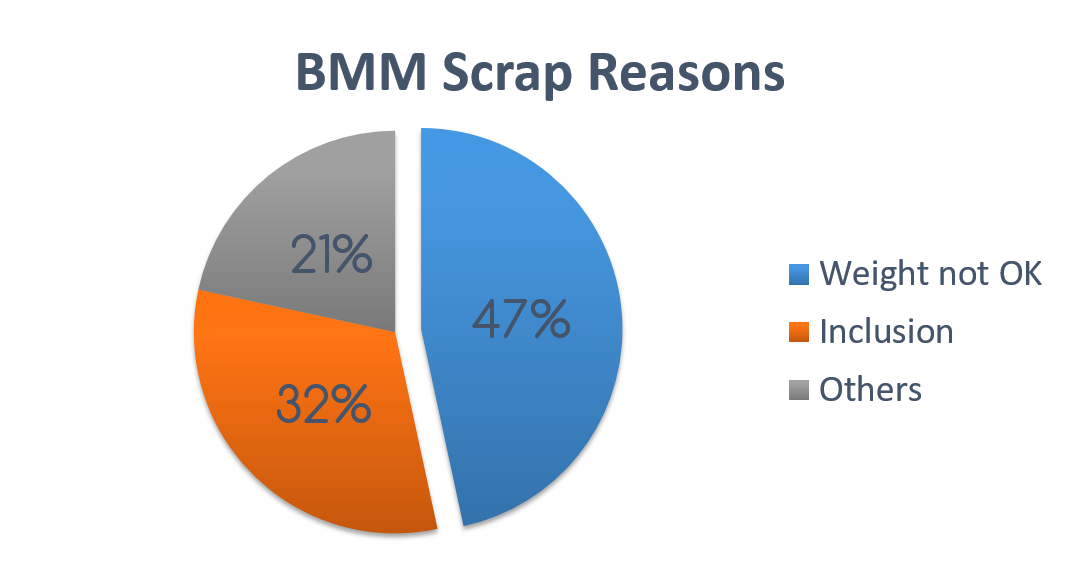
\includegraphics[scale=0.9]{images/chapter_3/Scraps_codes.eps}}
\caption{Most common scrap causes (2017--2019)}
\label{fig:Most common scrap causes (2017-2018-2019)}
\end{figure}

As a consequence of this analysis, we decided to focus our efforts on trying to understand where these scrap come from and what we can do to try to reduce them. By following the approach described in section \ref{Proposed Method} of this chapters, we aim to search for any hidden pattern or correlation within process data and quality data that could explain why some parts are not compliant in term of weight.


\subsection{Data collection TO BE FINISHED}

The industrial process taken into account has more than 5000 features measured in real-time by the PLC at each production cycle. Among all this features, 45 of them are considered as critical to ensure the proper process stability according to experts. Process parameters are stored in multiple databases and some pre-processing operations are needed to create a structured dataset.  Moreover, each process parameter measured in real-time during the production process has to be associated with the scalar value corresponding to the quality measurement of the manufactured product, at the end of the production cycle. In order to do that, some statistics (such as average, maximum and minimum) are calculated on the process parameters to have only scalar values.
Since the final parts are produced in batches of one or two days, we built our own dataset using data from 5 different batches, corresponding to as many production days, for a total of 5597 individuals. Some preliminary operations on features have been made to reduce the overall feature space: we used previous knowledge on the process to discard all features that cannot provide useful information. Moreover, in order to reduce multi-collinearity, we have deleted from the dataset some of the most highly correlated features. Finally, our dataset has a feature space of size 290. Data were normalized to have zero-mean and unit-variance. Standardizing the features is not only important if we are comparing measurements that have different units, but it is also a general requirement for many machine learning algorithms. 

Unfortunately, there is an important parameters that is not collected through the SCADA software, the parison length. As explained in section (add REF), the parison length provides information about the material distribution. Depending on the final length, the material distribution on the final tank may change and so the final tank weight. We therefore felt it was necessary to collect this additional data in order    

\subsubsection{Parison length estimation}

One of the key characteristic which can explain the tank weight variability is the length of the plastic parison when it is closed inside the molds at the beginning of the blow-molding process. In fact, accordingly to the length of the parison the distribution of the thickness may change and this can impact the weight of the final part. The parison length is not available within our process data database because the machine is not equipped with the sensors to measure it. Measuring the length of the parison requires to equip the machine with external sensors.
In order to be efficient, flexible and robust, our measuring system should present the following properties:

% TO BE REVIEWED
\begin{enumerate}
    \item Have a relatively small software and hardware cost compared to its manual counterpart.
    \item Require little to no expert intervention to adapt the model or process the data.
    \item Be rapidly adaptable to a novel or evolving industrial situation. The system should be easily adaptable to any blow-molding machine in every plant of the Company.
    \item Be capable of doing real time analysis.
    \item Be capable to return the result with a low latency.
    \item Be able to run in a hostile environment.
    \item Be robust to (small) variations in the environment (e.g. lighting).
\end{enumerate}

In order to respect the previous industrial constraints we made the choice to move towards a Computer Vision based approach. Our choice is motivated by the low cost of a camera, compared to others sensors, and by the performances achieved by deep-learning based algorithms in detecting object within images. The choice of working with deep  learning is motivated by the need of building a model able to infer the Parison length that is robust to the following challenges:

\begin{itemize}
    \item \textit{Scale Variation}
    \item \textit{Illumination conditions}
\end{itemize}

In section (ADD CHAPTER 2 SECTION) we shown how Neural Networks and, in particular, Convolutional Neural Networks reaches stet-of-the-art results in image based classification, object detection and image segmentation tasks. Motivated by the results presented in scientific literature we took the choice of train a Convolutional Neural Network able to detect the Parison in real-time and to provide the length measurement. In order to achieve real-time length detection we have chosen to compare the performances of two different Neural Networks architectures: \textit{SSD MobileNet-V2} architecture \citep{sandler2018mobilenetv2} and \textit{Faster R-CNN} \citep{ren2015faster}. MobileNet is an object detector released in 2017 as an efficient CNN architecture designed for mobile and embedded vision application. This architecture uses proven depth-wise separable convolutions to build lightweight deep neural networks. The choice of using these architecture is motivated by the the overall trade-off between the inference speed the model performances. Since we look for a real-time FINIRE  

The limited availability of data, 200 images are considered a really small dataset for deep-learning based computer vision tasks, this is why we decided to take advantage of a pre-trained Neural Network.

In order to train such a model, 200 parison images has been collected using a camera of HD resolution (1280x720). 

% Add parison images

Results has shown that MobileNet is able to provide accurate results within a limited amount of time. The computation time is less than 1 second on a \textit{Nvidia} Jetson Nano. Nvidia Jetson Nano is a small, powerful computer for embedded applications and AI IoT that delivers the power of modern AI. 


\begin{figure}
\centerline{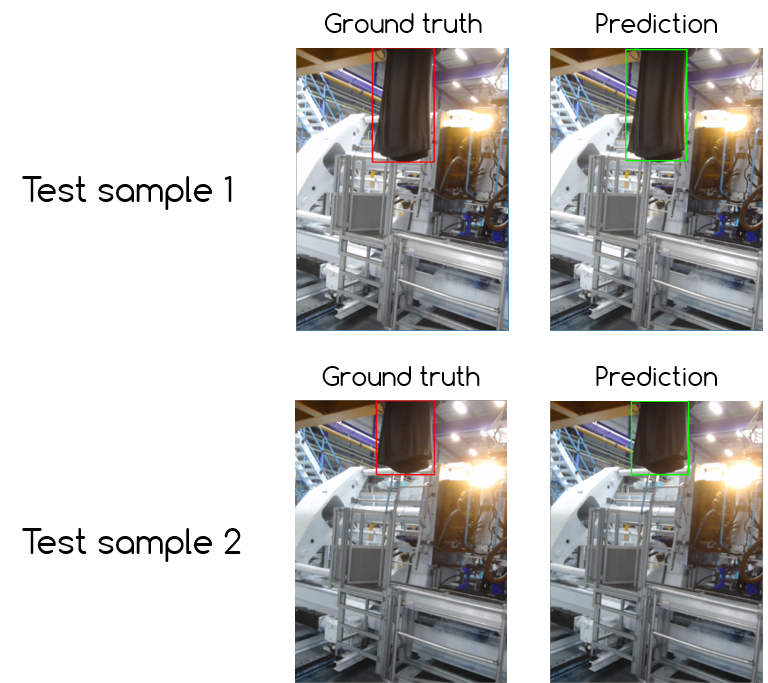
\includegraphics[scale=0.8]{images/chapter_3/parison_length_gt_prediction.png}}
\caption{Parison length inference example}
\label{fig:parison_inference}
\end{figure}

\subsection{Data processing TO BE FINISHED}

\subsubsection{The Human-based data cleaning TO BE FINISHED}

\subsubsection{The statistical data cleaning TO BE FINISHED}

\subsection{Exploratory data analysis TO BE FINISHED}



\subsection{Supervised learning modeling TO BE FINISHED}

\subsubsection{Training}

We compared multiple regressive models: Linear Regression, Lasso Regression, Ridge Regression, Random Forest and Gradient Boosting Tree. 

In order to evaluate the predictive power of our models, we used two different approaches: cross-validation and batch cross-validation. 

\paragraph{Batch cross validation}
Instead of performing the cross-validation on $k$ randomly split folds of the training set, we decided to split the whole dataset in the different batches (production days) and to cross-validate the model on each batch. Since in our dataset we have 5 different batches, at each time, one batch is used as a test set and the remaining 4 batches are used to fit the model.

\begin{equation}
    CV_{batch} = \frac{1}{n\degree\;batches}\sum_{i=1}^{n\degree\;batches}score_{i}
    \enspace.
\end{equation}

The mean of the 5 different scores is calculated to have an accurate estimate of the model prediction performance. With this strategy we want to know if the model built on multiple batches is capable to fit data belonging to an unseen batch.  

We used two different metrics: $R^2$ and the root mean squared error (RMSE). $R^2$, or coefficient of determination, is the proportion of the variance in the dependent variable that is predictable from the independent variable(s). Mathematically speaking, it can be expressed as follow:

\begin{equation}
    R^2 = 1 - \frac{RSS}{TSS}
    \enspace,
\end{equation}
where RSS is the residual sum of squares and TSS is the total sum of squares.
Values of the coefficient of determination range, normally, from zero (poor model) to one (perfect model) but can be negative if our model predicts our dependent variable worse than the mean of the independent variables. RMSE is the square root for the MSE (8) and it has the advantage of explaining the average model prediction error in units of measure of the variable of interest. 


\section{Results and Discussions TO BE FINISHED} \label{Results and Discussions}

The batch cross-validation $R^2$ is negative for all the statistical models applied on our dataset, which highlight how the dependent variable variability cannot be explained by our independent features. As it can be expected from looking at $R^2$, the RMSE score is far from being satisfactory regarding our needs. 
Results are quite astonishing but are showing evidence that it could be hard to apply statistical models in a field, manufacturing industry, where there is a lot of uncertainty. 
The impossibility of building a predictive model can be explained by multiple reasons:  

\begin{itemize}
    \item \textit{Non-stationarity of data}: results obtained with batch cross validation have shown how our models don’t generalise among different batches. Actually if we look at distributions of our input features we can see how they change considerably among different batches (Figure \ref{fig:Example of a process parameter variability in probability distribution}). A “Two-sample Kolmogorov-Smirnov” test has been applied on all two-pair batch combinations. Looking at results, only 35\% of the input features share the same probability distribution over all batches, with a 0.95 confidence level.
    \item \textit{Lack of data characterizing raw material properties}: the final part is the result of the transformation of raw material through our complex process. Unfortunately, to this date, these data are not available and they cannot be integrated in our dataset.
    \item \textit{Low variability in product quality}: given the already good performances of our process in term of capability, the variability of part in term of quality does not change too much. In most case the quality value range is quite limited and it becomes hard to have a high variability in the dataset.
    \item \textit{Reliability of the input data}: FINIRE
\end{itemize}

\begin{figure}
\centerline{\includegraphics[scale=0.4]{images/chapter_3/process_parameter.eps}}
\caption{Example of a process parameter variability in probability distribution}
\label{fig:Example of a process parameter variability in probability distribution}
\end{figure}

The Non-stationarity of the data depends FINIRE

The lack of data characterizing raw material properties FINIRE

Inbalanced dataset FINIRE



\section{SmartBMM: towards smarter machines TO BE FINISHED}

The data analysis results presented all along this chapter have shown the inability to explain the tank weight variability given the blow-molding process data that are considered as critical by the process experts. What the analysis has also highlighted is that the most of the scraps occurs just after the machine start-ups. As shown previously, right after the machine start-up, the extrusion blow-molding process is not completely stable which increase the overall scrap rate of the blow-molded parts. Moreover, an interview of different extrusion blow-molding experts has highlighted that there are not common and shared best practice to start the machine. As a consequence there is a lot of variability between startups.

\begin{figure}
\centerline{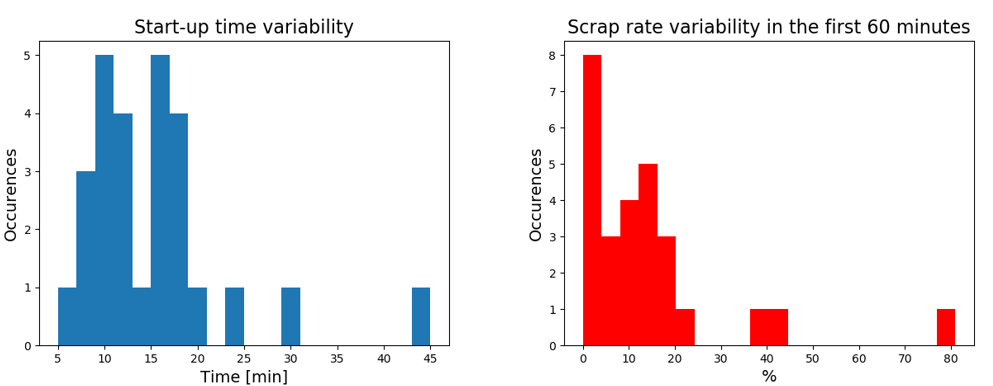
\includegraphics[scale=0.7]{images/chapter_3/smartbmm_barchart.png}}
\caption{Time and scrap rate variability for 27 machine start-ups in a Plastic Omnium plant}
\label{fig:smartbmm_barchart}
\end{figure}

In Figure \ref{fig:smartbmm_barchart} you could see an example of the previously described variability for 27 machine start-ups performed in a Plastic Omnium plant. On the left bar-chart, we can see how the time needed to start the machine may change from a start-up to another. Sometimes the start is done in 10 minutes, other times a full start may take around 15-20 minutes. In the same way, the right bar-chart highlights how the scrap rate in the first 60 minutes may change from a start up to another. Most of the time, hopefully, the scrap rate does not exceed the 5\%, but there are many starting for which the scrape rate value is above 10\% which is huge. 

Starting from these observations, it seemed necessary to us to put some efforts in trying to improve the way the blow-molding machines are started. We are aware the scraps may have a multitude of reasons which do not depends on the way the machine is started, but we claims that providing repeatable and optimized starting should benefit at the overall performance of the plant. 
The project was initially conceived to handle just the machine starting but it has been, later on, extended to also cover the Purge Out cycle of the machine. The reason is quite obvious, by ensuring good Purge cycles we can reduce the risk of incurring in contamination/inclusion problems. In this context, we have developed the \textit{SmartBMM} solution. \textit{SmartBMM} is a software which leverages the real-time data collected directly from the PLC of the machine and the past data to elaborate the best instructions to get the machine started without any manual intervention of the operators (Figure \ref{fig:SmartBMM}).

\begin{figure}
\centerline{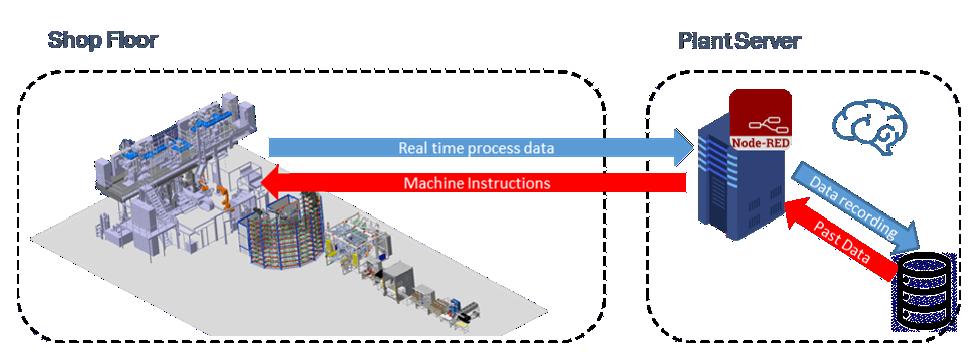
\includegraphics[scale=1]{images/chapter_3/SmartBMM.eps}}
\caption{\textit{SmartBMM} software}
\label{fig:SmartBMM}
\end{figure}

The previous representation shows broadly how the SmartBMM works. The SmartBMM software collect real time data from the PLC and store it in a database (\textit{InfluxDB}$^{\tiny{\textregistered}}$ database) in order to be able to retrieve it later. This steps is represented with the blue arrows. When the SmartBMM button is pressed the data collection continue, but, this time, the machine starts to write information to the PLC to get the machine started. The software takes the real time incoming data and the past data to elaborate the machine instructions to get the machine to the production conditions. Instead of manually start the machine by pressing simultaneously multiple buttons on the HMI (Human Machine Interface), machine setters and operators have to press only one button to start a cycle, whether it is a \textit{Starting} cycle or a \textit{Purge} cycle.  

\begin{itemize}
    \item The starting functionalities leverages the real-time data collected directly from the PLC of the machine and the past data to elaborate the best instructions to get the machine started without any manual intervention of the operators. The consecutive instructions FINIRE
    \item The Purge functionalities allows to improve the Purge cycles of the machine. There exist two Purge cycles: the Purge Out and the Purge In. The Purge Out cycle is done when the machine is stopped for more than 2 hours 
\end{itemize}

The interesting aspect of this project, apart from the benefits it brings to the process, is the way we have decided to pilot the machine. In fact, the logic that allows to perform the machine cycles is developed outside of the machine. extrusion blow-molding machines functioning, as well as for others industrial machines, is handled by an industrial PLC. 

We made the choice to develop the logic outside the PLC for two main reasons: 

\begin{itemize}
    \item Implementing the logic on an external system such as the “Edge Computing” platform reduce the number of PLC modifications of the machine. Our software is something non-intrusive. It is something which is plugged to the machine to introduce new functionalities.
    \item Developing complex logic which involves the communication with databases is by far more easy to do in a software such us Node-red compared to the PLC.
\end{itemize}

This strategy has, however, a main drawback. In fact, our tools completely rely on the plant network to communicate the instructions to the PLC. Which means that a bad network could be a bottleneck for the correct functioning of our software. Security features have been added on the software side to interrupt the communication with the machine if any network failures prevents to communicate with the machine.     


\section{Conclusion TO BE FINISHED}

In this chapter our approach for improving the process control has been presented. Firstly, we have proposed a general framework to model the relationship between the machine process data and the product quality of the part with the main purpose of understanding which parameters have an important influence on the quality of the finished part. Our data-driven approach requires 4 main stages: data acquisition, data processing, exploratory data analysis and machine learning modeling.  
In the second part of the current chapter, we have presented an empirical evaluation of our approach involving the industrial context in which this research work has been carried out. The results highlighted the impossibility to predict the tank weight using the data currently collected through the home made \textit{SCADA system}. Results are unexpected but are showing evidence that it could be hard to apply statistical models in a field, manufacturing industry, where there is a lot of uncertainty and where it is not possible to take into account all those elements that contribute to the variability of the part quality. Possible explanations of these results have been discussed as well as at the end of the Chapter.

\subsection{Scientific Contribution TO BE FINISHED}

Our main scientific contribution in this chapter



\subsection{Industrial Contribution}

This chapter has three main industrial contributions. Firstly, the work presented in this chapter has made it possible to call into question certain beliefs about the functioning of the blow-molding process. The critical process parameters considered as critical to ensure the correct functioning of the process do not allow to explain the tank weight variability. The control limits previously set for the critical parameters of the process, for ensuring the correct functioning of the production process, have proved to be insufficient to explain the tank weight variability. 

The Parison length measurement has opened new research perspectives. By measuring in real-time the length of the Parison, we will eventually be able to ensure the correct material distribution over the overall parison length. By ensuring the correct material distribution and by controlling the parison length we should be able to improve the process stability and, as a consequence, the quality of the manufactured parts. 

Finally, the \textit{SmartBMM} software that has been developed starting from the results obtained trough the data analysis process, has made it possible to improve the machine start-ups phases which are responsible for those transitional phases that lead to an higher scrape rate. By ensuring a faster and better start-up, we have proven to be able to shorten the duration of this transitional phase. By reducing the duration of the transitional phase it is possible to indirectly reduce the percentage of parts that do not comply with quality standards.   
Future works will make use of the parison length measured through the use of the camera to add to the SmartBMM software new functionalities to. 


